% !TEX program = xelatex
% !TEX encoding = UTF-8 Unicode

\documentclass[10pt]{beamer}
\usepackage{subfigure}
\usepackage{amssymb, amsmath, amsfonts,verbatim}
\usepackage{tikz, booktabs}
\graphicspath{ {./} }
\usetikzlibrary{matrix,arrows,fit,backgrounds,mindmap,plotmarks,decorations.pathreplacing}

\usepackage{pgfplots}
\pgfplotsset{compat=1.12}
\pgfdeclarelayer{background}
\pgfsetlayers{background,main}

\tikzset{decoration={name=none},}

\newlength\figureheight
\newlength\figurewidth

\newcommand{\tikzdir}[1]{#1.tikz}
\newcommand{\inputtikz}[1]{\input{\tikzdir{#1}}}

\newcommand{\tI}{\tilde {\mathcal I}}
\newcommand{\tA}{\tilde A}
\newcommand{\ty}{\tilde y}
\newcommand{\tx}{\tilde x}
\newcommand{\tw}{\tilde w}
\newcommand{\tv}{\tilde v}
\newcommand{\tC}{\tilde C}
\newcommand{\tP}{\tilde P}
\newcommand{\Ic}{{\mathcal I^c}}
\newcommand{\J}{{\mathcal J}}
\newcommand{\K}{{\mathcal K}}

\DeclareMathOperator{\pr}{Pr}
\DeclareMathOperator{\Smin}{Smin}
\DeclareMathOperator{\Smid}{Smid}
\DeclareMathOperator{\Smax}{Smax}
\DeclareMathOperator{\MSE}{MSE}
\DeclareMathOperator{\rank}{rank}
\DeclareMathOperator{\Med}{Med}
\DeclareMathOperator{\Max}{Max}
\DeclareMathOperator{\Min}{Min}
\DeclareMathOperator{\tr}{tr}
\DeclareMathOperator{\Cov}{Cov}
\DeclareMathOperator{\logdet}{log\;det}
\DeclareMathOperator{\argmin}{arg\;min}
\DeclareMathOperator{\argmax}{arg\;max}
\let\Tiny\tiny

\title[Secure Info Fusion]{Secure Information Fusion in Cyber-Physical Systems}
\author[Yilin Mo]{Yilin Mo}
\institute[Tsinghua]{
  Department of Automation\\ Tsinghua University\\
}
\date[Nov 21, 2019]{Nov 21st, 2019 \\ 
  \small Joint Work with Jiaqi Yan, Zishuo Li,\\
  Prof. Xiaoqiang Ren, Prof. Bruno Sinopoli, Prof. Joao Hespanha}

\usetheme[subsectionpage=none,block=fill]{metropolis}
\definecolor{thupurple}{RGB}{102,8,116}
\setbeamercolor{title separator}{fg=black!50}
\setbeamercolor{frametitle}{bg=thupurple!70!black}

\begin{document}

\maketitle 

\section{Introduction}

\begin{frame}{Cyber-Physical System}
  \begin{itemize}
  \item Cyber-Physical Systems (CPSs) refer to the embedding of computation, communication and control into physical spaces.
    \begin{center}
      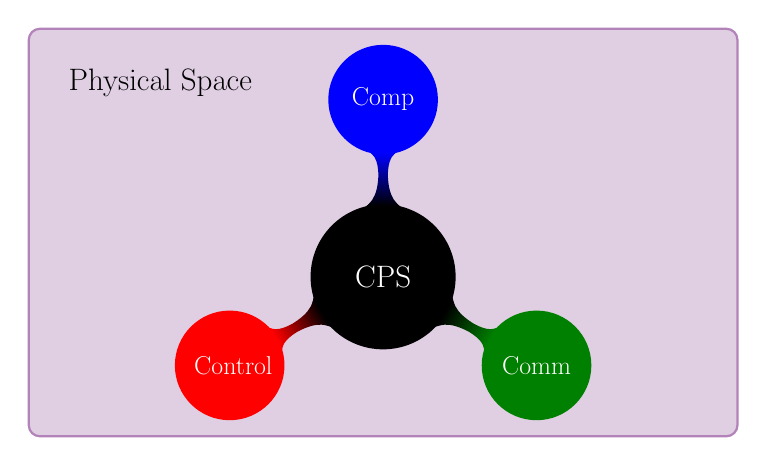
\begin{tikzpicture}[scale=0.45,transform shape,level distance=0cm,
        level 1 concept/.append style={sibling angle=120,minimum size = 3cm},
        ]
        \path [draw=thupurple!50,fill=thupurple!20,thick,rounded corners] (-10,-4.5) rectangle (10,7);
        \node at (-9,6) [anchor=north west] {\Huge Physical Space};
        \path[mindmap,concept color=black,text=white]
        node[concept] {\Huge CPS}
        [clockwise from=330]
        child[concept color=green!50!black] { node[concept](communication) {\huge Comm} }
        child[concept color=red] { node[concept](control) {\huge Control} }
        child[concept color=blue] { node[concept](computation) {\huge Comp} };
      \end{tikzpicture}
    \end{center}
  \item Applications: aerospace, chemical processes, civil infrastructure, energy, manufacturing and transportation. 
  \end{itemize}
\end{frame}

\begin{frame}{Security Threats for the CPS}
  \begin{itemize}
  \item The next generation CPS: Smart Grids, Smart Buildings, Smart Home, Internet of Things, will make extensive use of widespread sensing and networking.
  \item As the CPSs become ``smarter'', they are also more vulnerable to malicious attacks.
  \end{itemize}
  \begin{figure}[ht]
    \centering
    \includegraphics[width=0.6\textwidth]{SmartHome.jpg}
  \end{figure}
\end{frame}

\begin{frame}{Stuxnet}
  \begin{figure}[ht]
    \centering
    \includegraphics[width=0.8\textwidth]{stuxnet.jpg}
  \end{figure}
  Stuxnet is the first discovered malware that spies on and subverts industrial control systems. It was discovered in June 2010. 
\end{frame}

\begin{frame}{Industrial Control Systems}
  \begin{figure}[ht]
    \centering
    \includegraphics[width=0.6\textwidth]{cert.jpg}
  \end{figure}
  In FY 2016, ICS-CERT (Industrial Control Systems Cyber Emergency Response Team) received and responded to 290 incidents as reported by asset owners and industry partners.
\end{frame}

%\begin{frame}{Industrial Control Systems}
%  The scope of incidents encompassed a vast range of threats and observed methods for attempting to gain access to both business and control systems infrastructure, including but not limited to the following:
%  \begin{enumerate}
%  \item  Unauthorized access and exploitation of Internet facing ICS/Supervisory Control and Data Acquisition (SCADA) devices,
%  \item  Exploitation of zero-day vulnerabilities in control system devices and software, 
%  \item  Malware infections within air-gapped control system networks,
%  \item \dots
%  \end{enumerate}
%
%\end{frame}

\begin{frame}{Attack Through Compromised Supply Chain}
  \begin{figure}[ht]
    \centering
    \includegraphics[width=0.8\textwidth]{boeing.jpg}
    \caption{Boeing 787 outsourced 70\% of its parts.}
  \end{figure}
\end{frame}

\begin{frame}{2015 Ukraine Power Outage}
  \begin{figure}[<+htpb+>]
    \begin{center}
      \includegraphics[width=0.60\textwidth]{ukraine.jpg}
      \caption{A successful attack on CPS can have devastating effects.}
    \end{center}
  \end{figure}
\end{frame}

%\begin{frame}{What is New in CPS Security?}
%  Why not just use information security?
%  \begin{enumerate}
%  \item Physics
%  \item Physical Attacks: GPS Spoofing, etc.
%  \item Zero-day Attacks: Attack that exploits undiscovered vulnerabilities.
%  \item Cost: Securing every single device is difficult and costly
%  \item High reliability requirement
%  \end{enumerate}
%\end{frame}
%
%\begin{frame}{Defense in Depth}
%  \begin{figure}[<+htpb+>]
%    \begin{center}
%      \includegraphics[width=0.8\textwidth]{defense_in_depth.jpg}
%      \caption{Combining System Theory and Information Security to create better Protection for CPS}
%    \end{center}
%  \end{figure}
%\end{frame}

\begin{frame}{Hardening CPS Security using System Theory}
  \begin{itemize}
  \item System and Attack Modelling
  \item Intrusion Detection and Isolation
  \item Resilient Algorithm Design
  \item Fundamental Limitations
  \item Security System Design and Investment
  \item \dots
  \end{itemize}
\end{frame}

\section{Hypothesis Testing}

\begin{frame}{Static Detection Problem}
  \begin{itemize}
    \item We want to decide whether a binary state $\theta$ is $0$ or $1$.
    \item $m$ identical sensors are measuring the state: 
      \begin{center}
	\setlength{\figureheight}{3cm}
	\setlength{\figurewidth}{10cm}
	\inputtikz{gaussian}
      \end{center}
    \item The ``true'' measurements $z_i$ are independent and identically distributed.
  \end{itemize}
\end{frame}

\begin{frame}{Naive Bayes Detector}
  \begin{itemize}
    \item A detector is a function $f:\mathbb R^m\rightarrow \{-1,1\}$.
    \item The optimal detector (without attacks) with minimum detection error is a Naive Bayesian Detector:
      \begin{align*}
	\hat x=f(y)=\begin{cases}
	  -1 &\text{if }\sum_{i}z_i < 0\\
	  +1 &\text{if }\sum_{i}z_i \geq 0\\
	\end{cases}
      \end{align*}
    \item One corrupted measurement will possibly change the detection result. 
  \end{itemize}
\end{frame}

\begin{frame}{Byzantine Attack Model}
  \begin{itemize}
  \item The attacker can compromised $p$ sensors, the set of which is denoted as $\mathcal I$. 
    \begin{displaymath}
      y(k) = z(k) + a(k),  
    \end{displaymath}
    where $a_i(k) = 0$ if $i\notin \mathcal I$.
    \begin{center}
      \setlength{\figureheight}{2cm}
      \setlength{\figurewidth}{10cm}
      \inputtikz{blockdiagram}
    \end{center}
  \item The disturbance $a(k)$ depends $ Z(k)$ and $\mathcal I$: 
    \begin{displaymath}
      a(k) = g_k( Z(k),\mathcal I). 
    \end{displaymath}
  \item The attack strategy $g = (g_1,\,g_2,\,\dots)$.
  \item Assume that $p$ is less than half of $m$.
  \item The detector knows $p$, but does not know $\mathcal I$.
  \end{itemize}
\end{frame}

%
%\begin{frame}{Attack Model}
%  We assume the attacker knows the following:
%  \begin{itemize}
%    \item the detection algorithm $f$ (Kerckhoffs' Principle);
%    \item the true state $\theta$;
%    \item all measurements $z$.
%  \end{itemize}
%  The attacker can manipulate up to $p$ measurements arbitrarily.
%  \begin{displaymath}
%    z = y +  a, 
%  \end{displaymath}
%  where $a$ is $p$-sparse.
%
%  The attacker wants to maximize the probability of error:
%  \begin{displaymath}
%    P_e =\max_{\gamma\in S_\gamma,y^a} P(f(y^c)\neq x).
%  \end{displaymath}
%\end{frame}

%\begin{frame}{Attacker's Strategy}
%  The optimal strategy for the attacker:
%  \begin{align*}
%    (\gamma,y^a)= \begin{cases}
%      \displaystyle argmin_{\gamma\in S_\gamma, y^a} f(y+\gamma\circ y^a ) & (x =1)\\
%      \displaystyle argmax_{\gamma\in S_\gamma,y^a} f(y+ \gamma\circ y^a) & (x =-1)
%    \end{cases}
%  \end{align*}
%  \begin{figure}[<+htpb+>]
%    \centering
%    \subfigure[$x = -1$]{
%    \begin{tikzpicture}
%      \fill[red!20] (1.9,1.9)--(1.9,-1.9)--(-1.9,1.9);
%      \fill[green!20] (-1.9,-1.9)--(1.9,-1.9)--(-1.9,1.9);
%      \node at (1.9,1.9) [anchor = north east] {$\hat x = 1$};
%      \node at (-1.9,-1.9)[anchor = south west] {$\hat x = -1$};
%      \draw[->,thick] (-2,0)--(2,0) node [anchor = north]{$y_1$};
%      \draw[->,thick] (0,-2)--(0,2) node [anchor = west]{$y_2$};
%      \draw[thick,dashed] (-1,-1)--(-1,1.5);
%      \filldraw  (-1,-1) circle (2pt) node [anchor=east]{$y$};
%      \filldraw  (-1,1.5) circle (2pt) node [anchor=west]{$y^c$};
%    \end{tikzpicture}
%    }
%    \subfigure[$x = 1$]{
%    \begin{tikzpicture}
%      \fill[red!20] (1.9,1.9)--(1.9,-1.9)--(-1.9,1.9);
%      \fill[green!20] (-1.9,-1.9)--(1.9,-1.9)--(-1.9,1.9);
%      \node at (1.9,1.9) [anchor = north east] {$\hat x = 1$};
%      \node at (-1.9,-1.9)[anchor = south west] {$\hat x = -1$};
%      \draw[->,thick] (-2,0)--(2,0) node [anchor = north]{$y_1$};
%      \draw[->,thick] (0,-2)--(0,2) node [anchor = west]{$y_2$};
%      \filldraw  (-1,-1) circle (2pt) node [anchor=south]{$y=y^c$};
%    \end{tikzpicture}
%    }
%  \end{figure}
%\end{frame}
%
%\begin{frame}{Partitioning the Space of Measurements}
%  \begin{figure}[<+htpb+>]
%    \centering
%    \subfigure[First Detector $f_1$]{
%    \begin{tikzpicture}
%      \fill[red!20] (1.9,1.9)--(1.9,-1.9)--(-1.9,1.9);
%      \fill[green!20] (-1.9,-1.9)--(1.9,-1.9)--(-1.9,1.9);
%      \node at (1.9,1.9) [anchor = north east] {$\hat x = 1$};
%      \node at (-1.9,-1.9)[anchor = south west] {$\hat x = -1$};
%      \draw[->,thick] (-2,0)--(2,0) node [anchor = north]{$y_1$};
%      \draw[->,thick] (0,-2)--(0,2) node [anchor =north west]{$y_2$};
%      \filldraw  (-0.3,-0.3) circle (2pt) node [anchor=east]{};
%      \draw[dashed,thick] (-2,-0.3)--(2,-0.3);
%      \draw[dashed,thick] (-0.3,-2)--(-0.3,2);
%    \end{tikzpicture}
%    }
%    \subfigure[Second Detector $f_2$]{
%    \begin{tikzpicture}
%      \fill[green!20] (-1.9,-1.9)--(1.9,-1.9)--(1.9,1.9)--(-1.9,1.9);
%      \fill[red!20] (1.9,1.9)--(1.9,0)--(0,0)--(0,1.9);
%      \node at (1.9,1.9) [anchor = north east] {$\hat x = 1$};
%      \node at (-1.9,-1.9)[anchor = south west] {$\hat x = -1$};
%      \draw[->,thick] (-2,0)--(2,0) node [anchor = north]{$y_1$};
%      \draw[->,thick] (0,-2)--(0,2) node [anchor =north west]{$y_2$};
%      \filldraw  (-0.3,-0.3) circle (2pt) node [anchor=east]{};
%      \draw[dashed,thick] (-2,-0.3)--(2,-0.3);
%      \draw[dashed,thick] (-0.3,-2)--(-0.3,2);
%    \end{tikzpicture}
%    }
%  \end{figure}
%  There are three categories of point in $R^m$:
%  \begin{enumerate}
%    \item for some $\gamma\in S_\gamma,y^a$, $f(y+\gamma\circ y^a)=1$ and for some $\gamma\in S_\gamma,y^a$, $f(y+\gamma\circ y^a)=-1$. (Bad)
%    \item for all $\gamma\in S_\gamma,y^a$, $f(y+\gamma\circ y^a)=-1$. (\alert{Good})
%    \item for all $\gamma\in S_\gamma,y^a$, $f(y+\gamma\circ y^a)=1$. (\alert{Good})
%  \end{enumerate}
%\end{frame}
%
%\begin{frame}{Worst-Case Probability of Error}
%  Define
%  \begin{align*}
%    Y^-(f) &\triangleq \big\{y\in \mathbb R^m:f(y+\gamma\circ y^a)=-1, \; \forall y^a\in\mathbb R^m,\gamma\in S_\gamma\big\},\\
%    Y^+(f) &\triangleq \big\{y\in \mathbb R^m: f(y+\gamma\circ y^a)=1,\; \forall y^a\in\mathbb R^m,\gamma\in S_\gamma\big\}.
%  \end{align*}
%  The detector can correctly detect $x$ if and only if 
%  \begin{displaymath}
%    (x,y)\in\Big\{ (-1,y): y\in Y^-(f) \Big\} \cup \Big\{ (+1,y): y\in Y^+(f) \Big\}
%  \end{displaymath}
%  As a result, the worst-case probability of error is
%  \begin{displaymath}
%    P_e(f) = (1-\mu(Y^+(f)))p^+ +(1-\nu(Y^-(f)) p^-.
%  \end{displaymath}
%  If $Y^-(f)\subseteq Y^-(g)$ and $Y^+(f)\subseteq Y^+(g)$, then $P_e(f)\geq P_e(g)$.
%\end{frame}
%
%\begin{frame}{$Y^-$ and $Y^+$ for different detectors}
%  \begin{figure}[<+htpb+>]
%    \centering
%    \subfigure[First Detector]{
%    \begin{tikzpicture}
%      \fill[red!20] (1.9,1.2)--(1.9,-1.2)--(-1.9,1.2);
%      \fill[green!20] (-1.9,-1.2)--(1.9,-1.2)--(-1.9,1.2);
%      \node at (1.9,1.3) [anchor = north east] {$\hat x = 1$};
%      \node at (-1.9,-1.3)[anchor = south west] {$\hat x = -1$};
%      \draw[->,thick] (-2,0)--(2,0) node [anchor = north]{$y_1$};
%      \draw[->,thick] (0,-1.3)--(0,1.3) node [anchor =north west]{$y_2$};
%    \end{tikzpicture}
%    }
%    \subfigure[$Y^+$ and $Y^-$]{
%    \begin{tikzpicture}
%      \node at (1.9,1.3) [anchor = north east] {$Y^+ = \emptyset$};
%      \node at (-1.9,-1.3)[anchor = south west] {$Y^- = \emptyset$};
%      \draw[->,thick] (-2,0)--(2,0) node [anchor = north]{$y_1$};
%      \draw[->,thick] (0,-1.3)--(0,1.3) node [anchor =north east]{$y_2$};
%    \end{tikzpicture}
%    }\\
%    \subfigure[Second Detector]{
%    \begin{tikzpicture}
%      \fill[green!20] (-1.9,-1.2)--(1.9,-1.2)--(1.9,1.2)--(-1.9,1.2);
%      \fill[red!20] (1.9,1.2)--(1.9,0)--(0,0)--(0,1.2);
%      \node at (1.9,1.2) [anchor = north east] {$\hat x = 1$};
%      \node at (-1.9,-1.2)[anchor = south west] {$\hat x = -1$};
%      \draw[->,thick] (-2,0)--(2,0) node [anchor = north]{$y_1$};
%      \draw[->,thick] (0,-1.3)--(0,1.3) node [anchor =north west]{$y_2$};
%    \end{tikzpicture}
%    }
%    \subfigure[$Y^+$ and $Y^-$]{
%    \begin{tikzpicture}
%      \fill[green!80] (-1.9,-1.2)--(0,-1.2)--(0,0)--(-1.9,0);
%      \node at (1.9,1.2) [anchor = north east] {$Y^+ = \emptyset$};
%      \node at (-1.9,-1.2)[anchor = south west] {$Y^-$};
%      \draw[->,thick] (-2,0)--(2,0) node [anchor = north]{$y_1$};
%      \draw[->,thick] (0,-1.3)--(0,1.3) node [anchor =north east]{$y_2$};
%    \end{tikzpicture}
%    }
%  \end{figure}
%\end{frame}

\begin{frame}{A Hamming-like distance}
  Define metric $d:\mathbb R^m\times \mathbb R^m\rightarrow \mathbb N_0$ as
  \begin{displaymath}
    d(y_1,y_2)=\|y_1-y_2\|_0. 
  \end{displaymath}
  Let $Y_1,Y_2$ be two subsets of $\mathbb R^m$, define
  \begin{displaymath}
    d(Y_1,Y_2) = \min_{y_1\in Y_1,y_2\in Y_2}d(y_1,y_2),\,d(y,Y) =  \min_{y'\in Y}d(y,y').
  \end{displaymath}

%  \begin{lemma}
%    For any detector $f$, $d(Y^-(f),Y^+(f))\geq 2l+1$.
%  \end{lemma}
%  \begin{lemma}
%    Given $X^-,\,X^+$ two subsets of $\mathbb R^m$, and $d(X^-,X^+)\geq 2l+1$, there exists a detector $f$, such that $X^-\subseteq Y^-(f)$ and $X^+\subseteq Y^+(f)$.
%  \end{lemma}
\end{frame}

\begin{frame}{The structure of the optimal detector}
  \begin{theorem}
    The optimal $f^*$ is of the following form
    \begin{align*}
      f^*(y) = \begin{cases}
	1 & d(y,X^-)\ge d(y,X^+)\\
	-1 & d(y,X^-)< d(y,X^+),
      \end{cases}
    \end{align*}
    where $X^{+}$ and $X^{-}$ satisfies $d(X^+,X^-)\geq 2l+1$.
%    where $X^{+}$ and $X^{-}$  are the solutions of the following optimization problem:
%    \begin{align*}
%      &\mathop{\textrm{minimize}}\limits_{X^+,X^-}&
%      & (1-\nu(X^-))p^-+(1-\mu(X^+))p^+\\
%      &\textrm{subject to}&
%      & d(X^-,\,X^+)\geq 2l+1
%    \end{align*}
  \end{theorem}
\end{frame}

\begin{frame}{The structure of the optimal detector}
  \begin{figure}[<+htpb+>]
    \begin{center}
      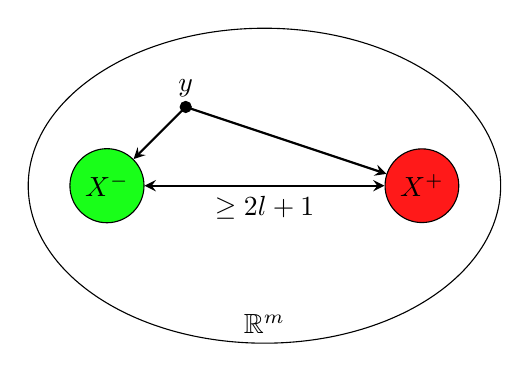
\begin{tikzpicture}
	\draw (0,0) ellipse (3 and 2);
	\node at (0,-2) [anchor = south] {$\mathbb R^m$};
	\node (xplus) at (-2,0) [circle,fill = green!90,draw] {$X^-$};
	\node (xminus) at (2,0) [circle,fill = red!90,draw] {$X^+$}
	edge [stealth-stealth,thick] node[auto] {$\geq 2l+1$} (xplus);
	\filldraw  (-1,1) circle (2pt) node [anchor=south]{$y$};
	\draw [-stealth,thick] (-1,1)--(xplus);
	\draw [-stealth,thick] (-1,1)--(xminus);
      \end{tikzpicture}
    \end{center}
  \end{figure}
  \begin{itemize}
    \item Directly working on the probability of error is hard.
    \item The exact optimal detection is very hard to compute in general.
  \end{itemize}
\end{frame}
%
%\begin{frame}{Optimal Detector for $m \leq 2l$ and $m = 2l+1$}
%  \begin{itemize}
%    \item If $m \leq 2l$, then the optimal detector is $f=1$ oare the solutions of the following optimization problem:r $f = -1$.
%    \item If $ m = 2l+1$, the optimal detector is based on voting:
%      \begin{enumerate}
%	\item The detector computes $m$ individual estimates $\hat x_i$ by a N-P detector based on individual measurements $y_i^c$:
%	  \begin{align*}
%	    \hat x_i \triangleq \begin{cases}
%	      -1 & \Lambda_{i}(y_i^c) <\eta_i\\
%	      1 & \Lambda_{i}(y_i^c) \geq\eta_i\\
%	    \end{cases}.
%	  \end{align*}
%	\item The detector decides $\hat x = 1$ if there are more than half of the $\hat x_i = 1$. Otherwise it decides $\hat x = -1$.
%      \end{enumerate}
%  \end{itemize}
%\end{frame}

\begin{frame}{Sequential Hypothesis Testing Problem}
  \begin{itemize}
    \item Let us define 
      \begin{displaymath}
	z(k) = \begin{bmatrix}z_1(k)&\dots&z_m(k)\end{bmatrix},\,Z(k) = \begin{bmatrix}z(1)&\dots&z(k)\end{bmatrix}.
      \end{displaymath}
    \item A detection strategy is an infinite sequence of detectors $f = (f_1,\,f_2,\,\dots)$, where each $f_k$ maps $Z(k)$ into a decison $\hat \theta(k)$.
    \end{itemize}
  \end{frame}

%\begin{frame}{A Classical Hypothesis Testing Problem}
% \begin{itemize}
%  \item Without the attacker, the optimal detector is a Naive Bayes Detector:
%    \begin{align*}
%      \hat \theta(k)=f_k(Z(k))=\begin{cases}
%        -1 &\text{if }\sum_{i=1}^m\sum_{t=1}^k z_i(t)/mk < 0\\
%        +1 &\text{if }\sum_{i=1}^m\sum_{t=1}^k z_i(t)/mk \geq 0\\
%      \end{cases}.
%    \end{align*}
%  \item However, it is not secure. 
%  \end{itemize}   
%\end{frame}

\begin{frame}{Performance: Probability of Error}
  \begin{itemize}
  \item The probability of error at time $k$ is denoted as
    \begin{displaymath}
      P_e(k) = \max_{\mathcal I,\theta}\; P(f_k(Y(k)) \neq \theta). 
    \end{displaymath}
  \item Clearly, $P_e(k)$ is a function of the detection strategy $f$ and the attack strategy $g$.
  \item  In general, for a fixed $k$, optimizing $P_e(k)$ directly (either from the system's perspective or the attacker's perspective) is difficult.
  \item As a result, we will focus on the asymptotic performance when $k\rightarrow\infty$.
  \end{itemize}
\end{frame}

\begin{frame}{Chernoff Information}
  \begin{itemize}
  \item Suppose we have a single benign sensor, the Naive Bayes Detector takes the following form:
    \begin{align*}
      \hat \theta(k)=f_k(Z(k))=\begin{cases}
        -1 &\text{if }\sum_{t=1}^k z_1(t)/k < 0\\
        +1 &\text{if }\sum_{t=1}^k z_1(t)/k \geq 0\\
      \end{cases}.
    \end{align*}
  \item By LLN, the probability of error goes to $0$.
  \item Moreover, it goes to $0$ exponentially fast, i.e.,
    \begin{displaymath}
      \lim_{k\rightarrow\infty}-\frac{\log P_e(k)}{k}= \frac{1}{2}.
    \end{displaymath}
  \item For multiple benign sensors, the probability of error for the Naive Bayes Detector satisfies:
    \begin{displaymath}
      P_e(k)\approx e^{-\frac{1}{2}mk}.
    \end{displaymath}
  \item For general pair of distributions, one can prove that $P_e \approx e^{-mCk}$, where $C$ is the Chernoff information between the two distributions.
  \end{itemize}
\end{frame}

\begin{frame}{Asymptotic Performance}
  \begin{itemize}
  \item In adversarial environment, let us define the rate function $I$ as
    \begin{displaymath}
      I = \liminf_{k\rightarrow\infty} -\frac{\log P_e(k)}{k}.
    \end{displaymath}
    Roughly speaking, 
    \begin{displaymath}
      P_e(k)\sim e^{-Ik}. 
    \end{displaymath}
    Larger rate implies better detection performance.
  \item  $I$ is a function of both detection strategy $f$ and attack strategy $g$.
  \item The detector wants to maximize $I$ while the attacker wants to minimize $I$.
  \end{itemize}
\end{frame}

\begin{frame}{``Optimal'' Attack Strategy $g^*$}
  \begin{itemize}
  \item Consider the attack, where the adversary simply flips the distribution of $p$ compromised sensors' measurements
    \begin{center}
      \inputtikz{attack}
    \end{center}
  \item The first $2p$ sensors have identical distribution.
  \item The only way to distinguish the two cases is to use the remaining $m-2p$ sensors.
  \item No detector can achieve a performance better than $(m-2p)C$ (Even if they know the adversary's strategy).
  \end{itemize}
\end{frame}

\begin{frame}{``Optimal'' Detection Strategy $f^*$}
  We need to define the following trimmed sum functions:
  \begin{definition}
    Define the symmetric functions $\Smin_{2p},\,\Smid_{2p},\,\Smax_{2p}:\mathbb R^{m}\rightarrow \mathbb R$ as  
    \begin{align*}
      \Smin_{2p}(y_1,\ldots,y_m) &\triangleq \sum_{i=1}^{m-2p}y_i,\\
      \Smid_{2p}(y_1,\ldots,y_m) &\triangleq \sum_{i=p+1}^{m-p}y_i,\\
      \Smax_{2p}(y_1,\ldots,y_m) &\triangleq \sum_{i=2p+1}^{m}y_i,
    \end{align*}
    when $y_1\leq \dots\leq y_m$.
  \end{definition}
\end{frame}

\begin{frame}{``Optimal'' Detection Strategy $f^*$}
  \begin{itemize}
  \item If $\|y - z\|_0\leq p$, then
    \begin{displaymath}
      \Smin_{2p}(z) \leq \Smid_{2p}(y)\leq \Smax_{2p}(z).
    \end{displaymath} 
  \item Assuming $m=5$, $p = 1$:
    \begin{center}
      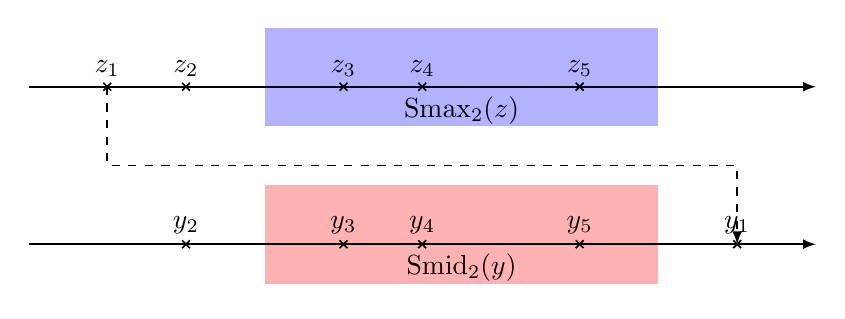
\begin{tikzpicture}[semithick,>=latex]
        \draw [->] (0,0)--(10,0);
        \draw plot[mark=x] coordinates{(1,0)} node [above] {$z_1$};
        \draw plot[mark=x] coordinates{(2,0)} node [above] {$z_2$};
        \draw plot[mark=x] coordinates{(4,0)} node [above] {$z_3$};
        \draw plot[mark=x] coordinates{(5,0)} node [above] {$z_4$};
        \draw plot[mark=x] coordinates{(7,0)} node [above] {$z_5$};
        
        \draw [->] (0,-2)--(10,-2);
        \draw plot[mark=x] coordinates{(9,-2)} node [above] {$y_1$};
        \draw plot[mark=x] coordinates{(2,-2)} node [above] {$y_2$};
        \draw plot[mark=x] coordinates{(4,-2)} node [above] {$y_3$};
        \draw plot[mark=x] coordinates{(5,-2)} node [above] {$y_4$};
        \draw plot[mark=x] coordinates{(7,-2)} node [above] {$y_5$};
        
        \draw [->,dashed] (1,0)--(1,-1)--(9,-1)--(9,-2);
        \begin{pgfonlayer}{background}
          \fill [fill=red!30] (3,-2.5) rectangle (8,-1.25);
          \node at (5.5,-2.3) {$\Smid_2(y)$};
          
          \fill [fill=blue!30] (3,-0.5) rectangle (8,0.75);
          \node at (5.5,-0.3) {$\Smax_2(z)$};
        \end{pgfonlayer}
      \end{tikzpicture}
    \end{center}
  \item $\Smid_{2p}$ is a more ``secure'' version of sum. 
  \item $\Smid_{2p}(y) < 0$ as long as $\Smax_{2p}(z)< 0$..
  \end{itemize}
\end{frame}

\begin{frame}{Equilibrium Strategies}
  \it Theorem: The following strategy pair $(f^*,g^*)$ forms a Nash-equilibrium with $I(f^*,g^*) = (m-2p)C$:
  \begin{block}{Attack Strategy $g^*$}
    Flip $p$ compromised sensors' measurements.
  \end{block}
  \begin{block}{Detection Strategy $f^*$}
    \begin{enumerate}
    \item For each sensor $i$, compute a local average $ \bar y_i(k) = \sum_{t=1}^k y_i(t)$.
    \item The detector $f_k$ is given by
      \begin{displaymath}
        f_k(Y(k)) = \begin{cases}
          -1 &\text{if }\Smid_{2p}(\bar y(k))< 0\\
          1 &\text{if }\Smid_{2p}(\bar y(k))\geq 0\\
        \end{cases}
      \end{displaymath}
    \end{enumerate}
  \end{block}
\end{frame}

\begin{frame}{What is the Cost of Security?}
  \begin{itemize}
  \item We need to consider the system performance both in the presence and in the absence of the attack.
    \vspace{0.5cm}
    \begin{center}
      \inputtikz{fun_lim2}
    \end{center}
  \item Unfortunately, trimmed sum has an efficiency of $(m-p)C$.
  \item How to get perfect security and efficiency simultaneously?
  \end{itemize}
\end{frame}

\begin{frame}{Cost-Free Security}
  \begin{enumerate}
  \item If there exists a set $J$ of $m-p$ sensors, such that
    \begin{align*}
      \sum_{i\in \mathcal J}\frac{1}{2}(\bar y_i+1)^2 < (m-2p)C,
    \end{align*}
    then choose $\hat \theta = 0$. 
  \item If there exists a set $J$ of $m-p$ sensors, such that
    \begin{align*}
      \sum_{i\in \mathcal J}\frac{1}{2}(\bar y_i-1)^2 < (m-2p)C,
    \end{align*}
    then choose $\hat \theta = 1$. 
  \item If none of the above conditions are satisfied, do a Naive Bayes test.
  \end{enumerate}
\end{frame}

\begin{frame}{Cost-Free Security}
  \begin{itemize}
  \item The best security $(m-2n)C$ and the best efficiency $mC$ are achieved simultaneously
  \item Security is ``cost-free''
    \begin{itemize}
    \item Computational burden: $O(m)$ versus $O(m\log m)$
    \end{itemize}
  \item Generalization: ``symmetric'' distributions. There exists a constant $a$ such that 
    \begin{align*}
      p_0(a+z) = p_1(a-z).
    \end{align*}
  \end{itemize}
\end{frame}

\begin{frame}{Generalization: Unknown Number of Compromised sensors}
  \begin{enumerate}
  \item Set $p = \lfloor m/2\rfloor -1$.
  \item 
    \begin{itemize}
    \item If there exists a set $J$ of $m-p$ sensors, such that
      \begin{align*}
        \sum_{i\in \mathcal J}\frac{1}{2}(\bar y_i+1)^2 < (m-2p)C,
      \end{align*}
      then choose $\hat \theta = 0$. 
    \item If there exists a set $J$ of $m-p$ sensors, such that
      \begin{align*}
        \sum_{i\in \mathcal J}\frac{1}{2}(\bar y_i-1)^2 < (m-2p)C,
      \end{align*}
      then choose $\hat \theta = 1$. 
    \end{itemize}
  \item Reduce $p$ by 1. If $p > 0$, go back to step 2, otherwise do a Naive Bayes test.
  \end{enumerate}
  The above algorithm is optimal for any number of compromised sensors.
\end{frame}

%\begin{frame}{General Case: Some Definitions from Large Deviation Theory}
%  \begin{center}
%    \inputtikz{rate_function}
%  \end{center}
%  \begin{itemize}
%  \item $I_\theta(y) \triangleq \sup_{w} yw - \log \mathbb E_\theta exp(\lambda w).$
%  \item $I_\theta(y)$ measures how typical a measurement $y$ is under each hypothesis.
%  \end{itemize}
%\end{frame}

\begin{frame}{General Cases}
  \begin{center}
    \inputtikz{fun_lim}
  \end{center}
  Fundamental Trade-off:
  \begin{align*}
I_0^{-1}\left(\frac{s}{m-n}\right)\leq I_1^{-1}\left(\frac{e}{m-n}\right),\, I_0^{-1}\left(\frac{e}{m-n}\right)\leq I_1^{-1}\left(\frac{s}{m-n}\right). 
  \end{align*}
  For the Gaussian case, the blue and red line will not cut the corner.
\end{frame}

\begin{frame}{General Case}
  The following detection strategy achieves the fundamental limit:
  \begin{enumerate}
  \item If there exists a set $J$ of $m-p$ sensors, such that
    \begin{align*}
      \sum_{i\in \mathcal J}I_0(\bar \lambda_i) < threshold,
    \end{align*}
    then choose $\hat \theta = 0$. 
  \item If there exists a set $J$ of $m-p$ sensors, such that
    \begin{align*}
      \sum_{i\in \mathcal J}I_1(\bar \lambda_i) < threshold,
    \end{align*}
    then choose $\hat \theta = 1$. 
  \item If none of the above conditions are satisfied, do a Naive Bayes test.
  \end{enumerate}
\end{frame}

\begin{frame}{Simulation}
  Assuming the following distribution:
  \begin{center}
    \begin{tabular}{@{}llr@{}}
      \toprule
      & $z = 0$ & $z=1$\\
      \midrule
      $\theta=0$ &0.98&0.02\\
      $\theta=1$ &0.4&0.6\\
      \bottomrule
    \end{tabular}
  \end{center}  
  We choose the detector with perfect efficiency:
  \begin{center}
    \inputtikz{finite_time}
  \end{center}
\end{frame}

\begin{frame}{Sequential Hypothesis Testing}
  Instead of deciding $\theta$ at a fixed time $t$, at every time, we can make 3 decisions:
  \begin{itemize}
    \item Decide $\theta = 0$;
    \item Decide $\theta = 1$; 
    \item Take another measurement.
  \end{itemize}

\end{frame}

\begin{frame}{Performance Metric}
  \begin{itemize}
    \item Similar to the previous case, we could define the rate function to be
    \begin{displaymath}
      I = \liminf_{P_e\rightarrow 0} -\frac{\log P_e}{\mathbb E T},
    \end{displaymath}
    where $P_e$ is a pre-specified probability of error and $T$ is the time to achieve such error.
  \item  $I$ is a function of both detection strategy $f$ and attack strategy $g$.
  \item The detector wants to maximize $I$ while the attacker wants to minimize $I$.
  \item Question: Does there exist a pair of equilibrium strategy $(f^*,g^*)$, such that
    \begin{displaymath}
      I(f^*,g)\geq I(f^*,g^*) \geq I(f,g^*).	
    \end{displaymath}
  \end{itemize}  
\end{frame}

\begin{frame}{Equilibrium Strategies}
  \begin{block}{Attack Strategy $g^*$}
    Flip $p$ compromised sensors' measurements.
  \end{block}
  \begin{block}{Detection Strategy $f^*$ (Vote Counting)}
    \begin{enumerate}
      \item Each sensor has two triggers $t_{i,0}=0$ and $t_{i,1}=1$.
      \item If $\sum_{t=1}^k y_i(t) < -threshold$ at certain time $k$, set $t_{i,0} = 1$
      \item If $\sum_{t=1}^k y_i(t) > threshold$ at certain time $k$, set $t_{i,1} = 1$
      \item Make a decision $\hat \theta = 0$ if $\sum_i t_{i,0} \geq m-p$, or $\hat \theta = 1$ if $\sum_i t_{i,1} \geq m-p$.
    \end{enumerate}
  \end{block}

  \begin{itemize}
      \item Only need to exchange at most $2m$ messages (regardless of $P_e$)
      \item Can be implemented as an event-based strategy.
      \item Potentially can be made into a distributed algorithm?
      \item Efficiency vs Security trade-off?
  \end{itemize}
\end{frame}

\section{Conclusion and Future Works}

\begin{frame}{Towards a Science of CPS Security}
  \begin{itemize}
    \item We consider both the hypothesis testing and the state estimation in adversarial environment and propose secure and efficient algorithm for both problems.
    \item System theory can help CPS to tolerate, detect and recover from malicious attacks.
    \item How to systematically design algorithms that are both secure and efficient?
    \item How to combine information security with system theory to provide defense in depth?
  \end{itemize}
\end{frame}

\begin{frame}[standout]
  Thank you!
\end{frame}

\end{document}
